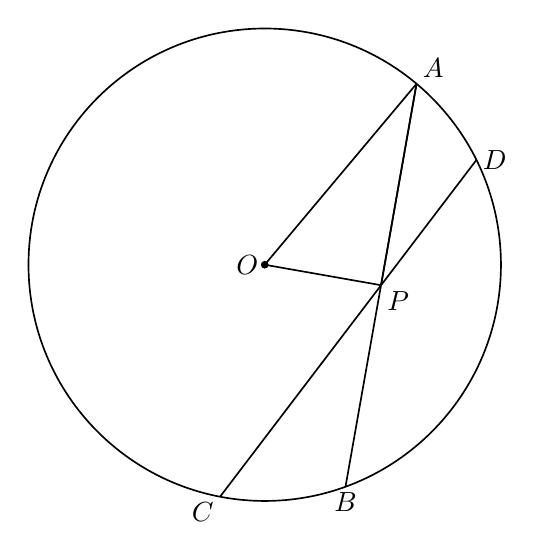
\begin{tikzpicture}[x=1cm,y=1cm,line width=.6pt,font=\normalsize]
\coordinate (O) at (0,0);
\coordinate (P) at (1.477,-0.26);
\coordinate (A) at (1.928,2.298);
\coordinate (B) at (1.026,-2.819);
\coordinate (C) at (-0.567,-2.946);
\coordinate (D) at (2.689,1.331);
\draw (O) circle[radius=3cm];
\draw (A)--(B);
\draw (C)--(D);
\draw (O)--(A);
\draw (O)--(P);
\draw (A)--(P);
\node[left=2pt,inner sep=0pt] at (O) {$O$};
\node[above right=2pt,inner sep=0pt] at (A) {$A$};
\node[below=2pt,inner sep=0pt] at (B) {$B$};
\node[below left=2pt,inner sep=0pt] at (C) {$C$};
\node[right=2pt,inner sep=0pt] at (D) {$D$};
\node[below right=2pt,inner sep=0pt] at (P) {$P$};

% Explicit named circle-center points, painted after all region fills.
\fill (O) circle[radius=1.4pt];
\end{tikzpicture}
